\begin{figure}[hbtp]
  \centering
  \subfigure[Disconnected isolated vertex]{
    \label{fig:subrefine-issue--1}
    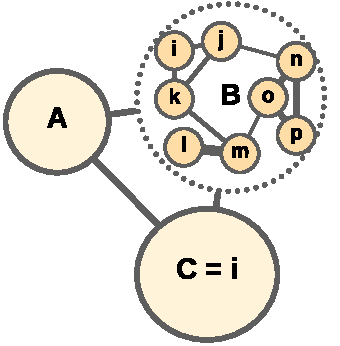
\includegraphics[width=0.45\linewidth]{out/subrefine-issue1.pdf}
  }
  \subfigure[Disconnected community formation]{
    \label{fig:subrefine-issue--2}
    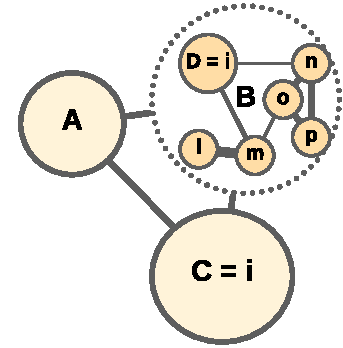
\includegraphics[width=0.45\linewidth]{out/subrefine-issue2.pdf}
  } \\[-1ex]
  \caption{Illustration of issues arising during the refinement phase when only a subset of communities is refined. Here, circles represent communities (or subcommunities after refinement), dotted circles indicate old parent communities (from the local-moving phase), and lines show both inter- and intra-community edges. Upon refinement of community $B$, subfigure (a) shows that vertex $i$ is isolated, but disconnected from community $C = i$, while subfigure (b) shows that further refinement forms sub-community $D = i$, which is disconnected from community $C = i$.}
  \label{fig:subrefine-issue}
\end{figure}
% Subfigure (a) demonstrates the isolation of vertex $i$ during selective refinement of community $B$, resulting in a disconnection from $C = i$. Subfigure (b) shows how further refinement can lead to the formation of two unconnected communities, $C = i$ and $D = i$, sharing the same ID. To resolve such inconsistencies, new IDs must be assigned to communities based on their constituent vertices, and associated data structures, including edge weights and flags, must be updated.
